% !TEX program = xelatex
% \DocumentMetadata{lang=en} % required for transparent package
\documentclass[10pt,aspectratio=169]{beamer}
\newcommand{\subhead}[1]{\flushleft {\bf\large #1}\\}

% remove footcite numbers
\makeatletter
\def\@makefnmark{}
\makeatletter

\setbeamersize{text margin left=5mm,text margin right=5mm} 

\newcommand\focus[1]{%
	{\alert{\textbf{#1}}}
}

\usepackage{amsthm,amsmath,amssymb,braket,fontspec,unicode-math,fontenc,libertine,pifont}
\usepackage[dvipsnames]{xcolor}
\usepackage[absolute,overlay]{textpos}

\graphicspath{{./figures/}}
\usetheme[nofirafonts,numbering=none]{focus}

% \setmainfont{Linux Libertine O}
% \setsansfont{Linux Libertine O}
\setmathfont{Fira Math}

\usepackage[backend=bibtex,url=false,doi=false,style=authoryear]{biblatex}
\setbeamertemplate{bibliography item}{}
\bibliography{bib}
\AtBeginBibliography{\scriptsize}

\AtBeginSection[]{}

\setbeamerfont{title}{size=\LARGE\scshape}
\setbeamerfont{author}{size=\Large}
\setbeamerfont{institute}{size=\large}
\setbeamerfont{date}{size=\large}
\setbeamerfont{frametitle}{size=\Large\scshape}
\setbeamerfont{sectiontitle}{size=\small\scshape}
\setbeamerfont{alerted text}{series=\bfseries}

\title{Mott Criticality as the Confinement \\ Transition of a Pseudogap-Mott Metal}
\subtitle{Presentation for Postdoctoral Position at ICTS-TIFR}

\author{Abhirup Mukherjee}

\institute
{
	Department of Physical Sciences,\\
	Indian Institute of Science Education and Research Kolkata
}
\date{January 7, 2026}
\titlegraphic{
	\vspace{80pt}
	\includegraphics[width=0.08\textwidth]{epqm_logo_mod.jpeg}\hspace*{20pt}\includegraphics[width=0.08\textwidth]{dps_logo.jpeg}\hspace*{350pt}
}

\begin{document}

\begin{frame}
    \titlepage
\end{frame}

\begin{frame}{A Brief Introduction}
	% \vspace{-60pt}
	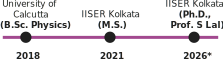
\includegraphics[width=0.55\textwidth]{education.pdf}
	\hfill
	\begin{minipage}{0.42\textwidth}
		\vspace{-40pt}
		\focus{Research Interests}
		\begin{itemize}
			\item Mott transition and criticality
			\item Unconventional superconductivity
			\item Kondo breakdown in heavy-fermion systems
			\item Various forms of quantum matter
		\end{itemize}
	\hspace{-20pt}
	\end{minipage}

	\focus{Skills and Techniques}
	\begin{itemize}
		\item Field theory (RG methods) and effective theory-based techniques
		\item \focus{Numerical computation} of correlation functions, entanglement measures, dynamical correlations (spectral function, self-energy, etc). Developed Python and \focus{Julia libraries} for the same.
		\item Developed \focus{new method} for using impurity models to analyse interacting lattice models
	\end{itemize}
\end{frame}

\begin{frame}{List of Projects}
\begin{itemize}
	\item[\ding{51}] {\bf Mott Criticality as the Confinement Transition of a Pseudogap-Mott Metal}. arXiv:2507.17201 (2025)\\[10pt]
	\item Revealing the magnetic dimensional crossover in the Heisenberg ferromagnet CrSiTe3 through picosecond strain pulses. Phys. Rev. B 111, L140414 (2025)\\[10pt]
	\item {\bf Holographic entanglement renormalisation for fermionic quantum matter}. J. Phys. A: Math. Theor. 57 275401 (2024)\\[10pt]
	\item {\bf Kondo frustration via charge fluctuations: a route to Mott localisation}. New J. Phys. 25 113011 (2023)\\[10pt]
	\item Frustration shapes multi-channel Kondo physics: a star graph perspective. J. Phys.: Condens. Matter 35 315601 (2023)\\[10pt]
	\item Unveiling the Kondo cloud: Unitary renormalization-group study of the Kondo model. Phys. Rev. B 105, 085119 (2022)
\end{itemize}
\end{frame}

\begin{frame}{A Note Of Thanks}
\begin{minipage}{0.18\textwidth}
	\centering
	\includegraphics[height=40pt]{slal.jpg}\\
	Prof. Siddhartha Lal (IISER K)
\end{minipage}
\hfill
\begin{minipage}{0.24\textwidth}
	\centering
	\includegraphics[height=40pt]{nsv.jpg}\\
	Prof. N. S. Vidhyadhiraja (JNCASR)
\end{minipage}
\hfill
\begin{minipage}{0.18\textwidth}
	\centering
	\includegraphics[height=40pt]{arghya.jpg}\\
	Prof. A. Taraphder (IIT KGP)
\end{minipage}
\hfill
\begin{minipage}{0.18\textwidth}
	\centering
	\includegraphics[height=40pt]{anamitra.png}\\
	Prof. A. Mukherjee (NISER)
\end{minipage}
\hfill
\begin{minipage}{0.18\textwidth}
	\centering
	\includegraphics[height=40pt]{IMSc.png}\\
	Prof. S. R. Hassan (IMSc)
\end{minipage}

\vfill
\begin{minipage}{0.5\textwidth}
\begin{itemize}
	\item SERB \& IISER Kolkata for funding
	\item PARAM RUDRA HPC facility for compute time
\end{itemize}
\end{minipage}
\hfill
\begin{minipage}{0.45\textwidth}
	\hfill
	\includegraphics[height=40pt]{iiserk.png}
	\hfill
	\includegraphics[height=40pt]{SERB.png}
	\hfill
\end{minipage}

\end{frame}

\section{\Large Mott Criticality as the Confinement Transition of a Pseudogap-Mott Metal}
\subsection{\large arXiv:2507.17201 (2025). Abhirup Mukherjee, S R. Hassan, A Mukherjee, N S. Vidhyadhiraja, A Taraphder, S Lal}

\begin{frame}{The Challenge: The Pseudogap and Strange Metal}
	\footcite{keimer2015quantum,ProustTaillefer2019,phillips2022,}

\vspace{-20pt}
\begin{itemize}
	\item Nature \& origin of pseudogap and strange metal phases of hole-doped Mott insulators
	\item Difficulty in understanding several puzzling experimental observations.
\end{itemize}

\vfill
\begin{center}
\hfill
\begin{minipage}{0.3\textwidth}
\centering
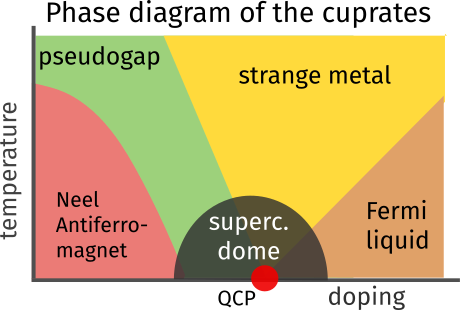
\includegraphics[height=0.6\textwidth]{cuprates.pdf}\\
Schematic {\bf High-Tc SC} Phase Diagram
\end{minipage}
\hfill
\begin{minipage}{0.35\textwidth}
\centering
\includegraphics[height=0.5\textwidth]{fermiArc1.png}\\
ARPES plot of {\bf Pseudogap}: gapped and gapless regions coexist
\end{minipage}
\hfill
\begin{minipage}{0.3\textwidth}
\centering
\includegraphics[height=0.6\textwidth]{linearResis.jpg}\\
Linear Resistivity in {\bf Strange Metal} crosses MIR bound
\end{minipage}
\hfill
\end{center}
\vfill

\visible<2>{
\begin{itemize}
	\item Pseudogap a \focus{precursor} to Mott insulator/ Superconductor? Nature of its excitations?
	\item Which metal is \focus{parent phase} of Mott insulator, \focus{at \(1/2-\)filling}?
	\item Is strange metal a new scale-invariant \focus{long-range entangled} strongly interacting phase?
\end{itemize}
}
\end{frame}

\begin{frame}{Our Approach, In a Nutshell}
	\footcite{stoyanova,anirbanurg1,anirbanurg2,Mukherjee_2023}
	\begin{minipage}{0.45\textwidth}
		\includegraphics[width=\textwidth]{tilingNUtshell.pdf}
	\end{minipage}
	\hfill
	\begin{minipage}{0.45\textwidth}
	Solve an \alert{impurity model} \(H_\text{imp}\) with certain properties:
	\begin{itemize}
		\item Lattice symmetry
		\item Localisation transition
	\end{itemize}~\\
	\focus{Construct correlated lattice} model by applying many-body translation operators (``tiling")
	\begin{itemize}
		\item Restore discrete translation invariance
	\end{itemize}~\\
	Analyse impurity mode using \focus{unitary RG}* method.\\

	Tile with \focus{fixed-point impurity model} for low-energy properties of lattice model.
	\end{minipage}

\end{frame}

\begin{frame}{The Core Ingredient: A Lattice-Embedded Impurity Model}
% \footcite{Yang2002}

\begin{minipage}{0.65\textwidth}
Lattice-variant of extended Anderson impurity model
\vspace{10pt}
\begin{itemize}
	\item {\color{Maroon}\bf Red site}: correlated impurity site (strong local \(U\))
	\item {\color{Violet}\bf Rest of the sites}: conduction bath (hopping \(t\))
	\item Impurity-bath hybridisation: \focus{Kondo} \(J\), hopping \(V\)
	\item Weak \focus{local interaction} \(W\) on N.N bath sites
\end{itemize}

\vspace{10pt}
For \(U \gg V\), Mott transition driven by \(J\) and \(W\)\footnotemark**

\end{minipage}
\begin{minipage}{0.3\textwidth}
	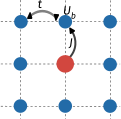
\includegraphics[width=\textwidth]{pWaveEsiam.pdf}
\end{minipage}

\visible<2>{
\[H_\text{aux} = H_\text{coup} + H_\text{cbath}\]
\[H_\text{cbath} = \sum_{k,\sigma}\epsilon_k n_{k,\sigma} -\frac{W}{2}\sum_{Z} \left(n_{Z\uparrow} - n_{Z\downarrow}\right)^2,\quad Z = \text{N.N}\]
\[H_\text{coup} = J\sum_{Z} {\bf S}_d\cdot {\bf S}_Z,\quad J_{k,k^\prime} = \frac{J}{2}\left[\cos(k_x-k_x^\prime) + \cos(k_y-k_y^\prime)\right]\]
}
\footnotetext[1]{**Observed in ∞-dimensional problem: Mukherjee et al., NJP (2023)}

\end{frame}

\begin{frame}{Tiling from Impurity Model to Two Dimensions}
“Tiling” allows us to translate physics obtained by from the impurity model into that of the 2D extended Hubbard model
\vfill
\begin{center}
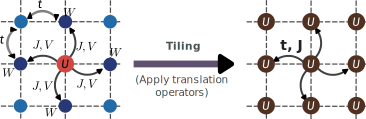
\includegraphics[width=0.8\textwidth]{tilingHamiltonian.pdf}
\end{center}
\vfill

\begin{minipage}{0.65\textwidth}
\focus{Reconstructed lattice Hamiltonian:}
\[-\frac{\tilde t}{\sqrt{\mathcal{Z}}} \sum_{\left<{\bf r}_i, {\bf r}_j\right>;\sigma}\left(c^\dagger_{{\bf r}_i,\sigma}c_{{\bf r}_j,\sigma} + \text{h.c.}\right) + \frac{\tilde J}{\mathcal{Z}}\sum_{\left< {\bf r}_i, {\bf r}_j\right>}{\bf S}_{{\bf r}_i}\cdot{\bf S}_{{\bf r}_j} - \frac{1}{2}\tilde U\sum_{\bf r}\left(\hat n_{{\bf r} , \uparrow} - \hat n_{{\bf r} , \downarrow}\right)^2
\]
\end{minipage}
\begin{minipage}{0.3\textwidth}
	\[\tilde t = 2V/Z\]
	\[\tilde U = U + W\]
	\[\tilde J = 2J/Z\]
\end{minipage}
\end{frame}

\begin{frame}{Unitary Renormalisation Scheme}
\footcite{anirbanurg1,anirbanurg2}
\hfill
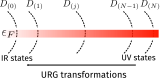
\includegraphics[width=0.35\textwidth]{urg-scheme.pdf}
\hfill
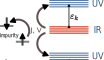
\includegraphics[width=0.4\textwidth]{urgProcesses.pdf}
\hfill

\vfill
\centering
\hfill
\begin{minipage}{0.25\textwidth}
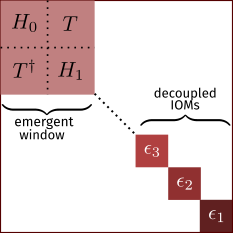
\includegraphics[width=\textwidth]{urg_ham_full.pdf}
\end{minipage}
\hfill
\begin{minipage}{0.5\textwidth}
	\begin{itemize}
		\item Wanted: \focus{low energy theory}
		\item RG procedure accounts for non-trivial scattering into various energy sectors
		\item RG proceeds via decoupling of high energy degrees of freedom via many-body \focus{unitary} transformations
	\end{itemize}
\end{minipage}
\hfill
\end{frame}

\begin{frame}{Unitary RG Phase Diagram and Pseudogapping Transition}
\begin{minipage}{0.5\textwidth}
	\focus{Competition} between Kondo coupling and local interaction on bath sites:
\[\Delta J^{(j)}_{{\bf k}_1, {\bf k}_2} = -2\sum_{{\bf q}} \frac{J^{(j)}_{{\bf k}_2,{\bf q}} J^{(j)}_{{\bf q},{\bf k}_1} + 4J^{(j)}_{{\bf q}, {\bf \bar q}} W_{{\bf \bar q}, {\bf k}_2, {\bf k}_1, {\bf q}}}{\omega - \frac{1}{2}|\varepsilon_j| + J^{(j)}_{{\bf q}}/4 + W_{{\bf q}}/2}\]
\end{minipage}
	\hfill
\begin{minipage}{0.25\textwidth}
	\centering
	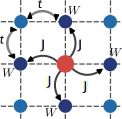
\includegraphics[width=\textwidth]{Jub.pdf}
\end{minipage}
	
\begin{center}
	\begin{minipage}{0.35\textwidth}
	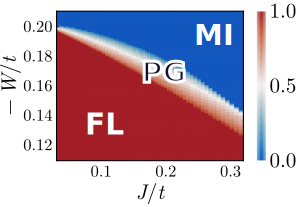
\includegraphics[width=\linewidth]{phaseDiagram.pdf}
	\end{minipage}
	\hfill
	\begin{minipage}{0.6\textwidth}
	\begin{itemize}
		\item Competition leads to \focus{Kondo breakdown} for $W<0$
		\item Phase diagram shows \focus{pseudogap} phase lying between Fermi liquid (FL) and Mott insulator (MI).
		\item PG possesses non-Fermi liquid excitations -- a \focus{Mott Metal}
	\end{itemize}
	\end{minipage}
\end{center}
\end{frame}

\begin{frame}{Journey Into The Pseudogap}
	\begin{itemize}
		\item Strength of Landau quasiparticle excitations of FL (\focus{QP residue} Z) vanishes upon entering PG.
		\item Impurity magnetisation \(\langle S_d^z \rangle\) grows dramatically in PG: \focus{breakdown} of Kondo screening.
		\item Impurity spectral function shows \focus{pseudogap} at \(\omega=0\)!
	\end{itemize}
	\vfill
	
	\includegraphics[width=0.32\textwidth]{QPR_77-1500.pdf}
	\includegraphics[width=0.32\textwidth]{sdz_77-1500.pdf}
	\includegraphics[height=0.25\textwidth]{Ad_zoomin_77-1500.pdf}
\end{frame}

\begin{frame}{Luttinger Surfaces in the Pseudogap}
	\footcite{keimer2015quantum}
	\begin{minipage}{0.75\textwidth}
	\begin{itemize}
		\item PG shows \focus{electronic differentiation} in lattice spectral function: gapped antinodal regions (\focus{Luttinger surfaces}), gapless excitations in nodal regions.
		\item Electron \focus{scattering rate}  shows divergences in gapped antinodal regions, while it is analytic in gapless nodal regions.
		\item \( 1/\Sigma^{\prime\prime} \sim 1/\Sigma^{\prime\prime}_0 + \omega^2\). Appearance of power-law exponents such as 2 signals \focus{universality}.\\[10pt]
	\end{itemize}
	\end{minipage}
	\hfill
	\begin{minipage}{0.2\textwidth}
	\includegraphics[width=\textwidth]{fermiArc1.png}
	\end{minipage}
	\vfill
	
	\centering
	\includegraphics[height=0.25\textwidth]{kspaceDOS-77.pdf}
	\hfill
	\includegraphics[height=0.25\textwidth]{selfEnergyKspace.pdf}
	\hfill
	\includegraphics[height=0.22\textwidth]{selfEnergy_d_fit_77-1500.pdf}
\end{frame}

% \begin{frame}{Universal Scaling of Spectral Features}
% 	\begin{itemize}
% 		\item Electron Scattering Rate of NFLs cross \focus{Mott-Ioffe-Regel (MIR) bound} (no electron-like excitations!), while FLs are within it.\\[10pt]
% 		\item \( 1/\Sigma^{\prime\prime} \sim 1/\Sigma^{\prime\prime}_0 + \omega^2\). Appearance of power-law exponents such as 2 signals \focus{universality}.\\[10pt]
% 		\item Optical Conductivity \(\sigma \sim A(\omega) \tau(\omega)\) shows a \focus{shifted ``Drude" peak}
% 	\end{itemize}
% 	\vfill
%
% 	\centering
% 	\hfill
% 	\includegraphics[height=0.22\textwidth]{selfEnergy_d_zoomin_77-1000withMIR.pdf}
% 	\hfill
% 	\includegraphics[height=0.22\textwidth]{selfEnergy_d_fit_77-1500.pdf}
% 	\hfill
% 	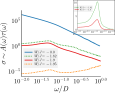
\includegraphics[height=0.22\textwidth]{sigma_in.pdf}
% 	\hfill
% \end{frame}

\begin{frame}{Long-ranged and Multipartite Entanglement in the PG}
\begin{itemize}
	\item real-space correlations and entanglement undergo a crossover within the pseudogap from short-ranged to \focus{long-ranged} behaviour\\[10pt]
	\item Quantum Fisher information for \(\mathcal{O} = \sum_{\text{odd}~i}(S_i^+ S_{i+1}^- + \text{h.c.})\) shows a jump in \focus{multipartite entanglement} of 2 in FL to 5 within PG. \\[10pt]
	\item Densely entangled \focus{Quantum Soup}!
\end{itemize}

\begin{center}
	\includegraphics[height=0.25\linewidth]{SF-di_77-700.pdf}
	\includegraphics[height=0.25\linewidth]{I2-di_77-700.pdf}
	\includegraphics[height=0.25\linewidth]{qfi_77-2000.pdf}
\end{center}
\end{frame}

\begin{frame}{Singular Nodal Metal at Critical Point}
\begin{minipage}{0.65\textwidth}
\begin{itemize}
	\item Mott critical point has \focus{nodal non-Fermi liquids}. Theory can be obtained in the form of exactly solvable \focus{Hatsugai-Kohmoto model}!
		\[H_\text{eff} = \sum_{{\bf q}, \sigma}\epsilon_{\bf q} r_{{\bf q},\sigma} + \mathcal{U}\sum_{{\bf q}, \sigma}r_{{\bf q} \sigma}r_{{\bf q} \bar\sigma}\]
		\[\quad r_{{\bf q} \sigma}:~\text{nested combination across FS}\]
	\item Nodal metal is singular, i.e., has a Mott pole in self-energy at Fermi energy, but is still gapless. Gapless excitations are \focus{holons \& doublons}.\\[10pt]
\end{itemize}
\end{minipage}
\hfill
\begin{minipage}{0.3\textwidth}
	
\includegraphics[width=\textwidth]{nodalMetal.pdf}
\end{minipage}

\end{frame}

\begin{frame}{Conclusions: Main Takeaways}
\begin{minipage}{0.5\textwidth}
Realisation of \focus{Mott’s original vision} (1949) with deconfined holes \& doubles
\begin{itemize}
	\item new, (likely) universal phase of \focus{strongly interacting} quantum matter,\\[10pt]
	\item \focus{noisy}, incoherent environment for electron-like excitations,\\[10pt]
	\item a long-ranged and \focus{multipartite} entangled “quantum soup”,\\[10pt]
	\item scale invariant at Mott critical point \& described by exactly solvable model\\[10pt]
\end{itemize}
\focus{Open Questions:}\\
Fate at non-zero temperatures, doping, other geometries?
\end{minipage}
\hfill
\begin{minipage}{0.49\textwidth}
	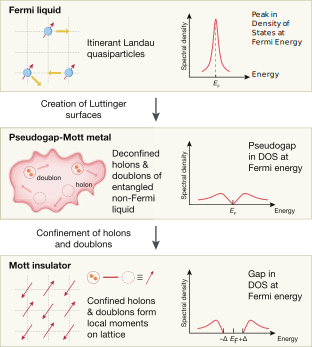
\includegraphics[width=\textwidth]{results.pdf}
\end{minipage}
\end{frame}

\begin{frame}{Brief Mentions of Other Projects}
\focus{Kondo frustration via charge fluctuations: a route to Mott localisation}\\
{\bf New J. Phys. 25 113011 (2023)}. {\bf Abhirup Mukherjee}, N S. Vidhyadhiraja, A Taraphder, S Lal\\
Precursor to the Mott metal work. Demonstrated how an extended Anderson impurity model captures the \(d=\infty\) Mott MIT on the Bethe lattice.
\vfill

\focus{Holographic entanglement renormalisation for fermionic quantum matter}\\
{\bf J. Phys. A: Math. Theor. 57 275401 (2024)}. {\bf Abhirup Mukherjee}, S Patra, S Lal\\
Demonstration of the holographic principle by showing how entanglement renormalisation in a free fermion system leads to a holographic dimension.
\vfill

\focus{Revealing the magnetic dimensional crossover in the Heisenberg ferromagnet CrSiTe3 through picosecond strain pulses}\\
{\bf Phys. Rev. B 111, L140414 (2025)}. A Kumar N M, S Mukherjee,{\bf Abhirup Mukherjee}, A Punjal, S Purwar, T Setti, S Prabhu S., S Lal, N Kamaraju\\
Investigated the two-step magnetic dimensional crossover in CrSiTe3. We came up with a simple Ginzburg-Landau model of phonons interacting with the lattice spin fluctuations to explain the softening/gapping of various phonon modes observed from a pump-probe experiment.
\end{frame}

\begin{frame}{Brief Mentions of Other Projects}
\focus{Frustration shapes multi-channel Kondo physics: a star graph perspective}\\
{\bf J. Phys.: Condens. Matter 35 315601 (2023)}. S Patra, {\bf Abhirup Mukherjee}, A Mukherjee, N S Vidhyadhiraja, A Taraphder, S Lal\\
We investigated the single-channel Kondo model and demonstrated the presence of two-particle correlations and entanglement within the Kondo cloud in the form of an effective Hamiltonian; we also calculated how they evolved during the high to low-temperature crossover.

\vfill
\focus{Unveiling the Kondo cloud: Unitary RG study of the Kondo model}\\
{\bf Phys. Rev. B 105, 085119 (2022)}. A Mukherjee, {\bf Abhirup Mukherjee}, N S. Vidhyadhiraja, A Taraphder, S Lal\\
Shed light on the role played by the ground state degeneracy in the non-Fermi liquid physics - how it
leads to an orthogonality catastrophe in the low-energy excitations and how it modified the various correlations into anomalous forms.
\end{frame}

\begin{frame}{Future Interests}
	\vspace*{-20pt}
	\begin{itemize}
		\item Investigations into \focus{quantum critical/non-Fermi liquid} behaviour in correlated models (randomness, heavy-fermions, etc)\\[10pt]
		\item \focus{Spin liquids}: Phase transitions, nature of entanglement, etc\\[10pt]
		\item Topological phases of matter
	\end{itemize}
	
	\vfill
	\centering
\hrule  height 2pt
\vspace{2em}
\focus{\Large Thank You}

\end{frame}

\begin{frame}{Mott MIT as holon-doublon deconfinement}
\footcite{Mott_1949}
The Mott MIT is essentially a holon-doublon \focus{binding-unbinding} transition
\vfill
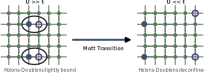
\includegraphics[width=\textwidth]{mottPicture.pdf}
\vfill
\begin{itemize}
	\item Delocalised \focus{gas of holons \& doublons} form metal: Fermi liquid?
	\item Nature and mechanism of transition?
\end{itemize}
\end{frame}

\section{\Large The single-channel Kondo problem: Anatomy of the Kondo cloud\vspace*{10pt}}
\begin{textblock*}{\textwidth}(1cm, 5cm)
\large \bf Anirban Mukherjee et al., Phys. Rev. B 105, 085119
\end{textblock*}
\subsection{~}

\begin{frame}{Effective Hamiltonian for the Kondo cloud}
\footcite{anirban_kondo,anirbanurg1,anirbanurg2}
We first applied the \alert{unitary RG} to obtain a low energy fixed point theory.\\[10pt]
To obtain a theory for the Kondo cloud, we \alert{trace out impurity} from fixed point Hamiltonian.
\vspace*{\fill}

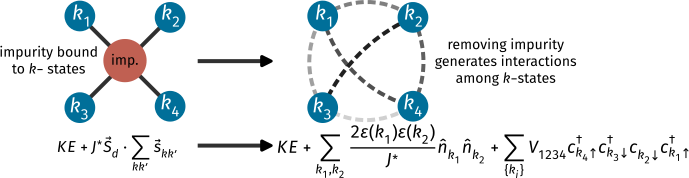
\includegraphics[width=\textwidth]{KondoCloud.pdf}

\vspace*{\fill}
\begin{itemize}
	\item all-to-all interactions between momentum states, \alert{large entanglement}
	\item 2-particle interaction terms \alert{not} present in Fermi liquid, are \alert{responsible for screening}
\end{itemize}

\end{frame}

\begin{frame}{Quantifying entanglement within the Kondo cloud}
\footcite{anirban_kondo}
In order to demonstrate formation of Kondo cloud, we study the \alert{variation of entanglement} and correlations under RG transformations.

\vspace*{\fill}
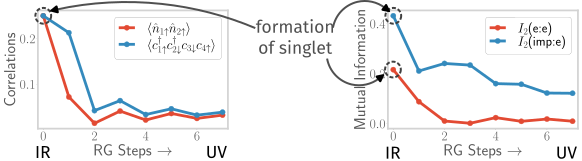
\includegraphics[width=\textwidth]{kondoRevRG.pdf}

\vspace*{\fill}
\begin{itemize}
	\item Both entanglement and \(k-\)space correlations \alert{increase} as RG proceeds from UV to IR.\\[10pt]
	\item This shows the formation of the \alert{Kondo singlet} and the growth of two-particle correlations in the \alert{Kondo cloud}.
\end{itemize}
\end{frame}

\section{\Large Distorting the Kondo singlet: The multi-channel Kondo Problem\vspace*{10pt}}
\begin{textblock*}{\textwidth}(1cm, 5cm)
\large \bf Siddhartha Patra et al., 2023 J. Phys.: Condens. Matter 35 315601
\end{textblock*}
\subsection{~}

\begin{frame}{What is the multichannel Kondo problem?}
\footcite{Noz_blandin_1980,affleck1993exact,emery_kivelson,andrei_destri_1984}
\begin{minipage}{0.39\textwidth}
Single impurity interacting with \alert{multiple channels} in the bath
\[H_\text{Kondo} = KE_\text{bath} + \sum_{l}J_l \vec{S}_\text{imp}\cdot\vec{s}^{(l)}\]
\end{minipage}
\hspace*{\fill}
\begin{minipage}{0.59\textwidth}
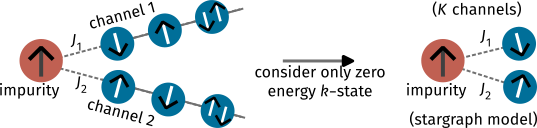
\includegraphics[width=\textwidth]{MCKM_zeroB.pdf}
\end{minipage}\\[10pt]
Known to display divergent \(T=0\) impurity susceptibility (incomplete screening), and orthogonality catastrophe, \alert{non-Fermi liquid} excitations.\\[10pt]
\begin{minipage}{0.64\textwidth}
Zero bandwidth limit is (analytically) solvable: \(\left\{\ket{S_\text{tot}^z}\right\}\)\\
\begin{itemize}
	\item Ground state degeneracy for \(K > 1\) explains \alert{orthogonality catastrophe}\\[5pt]
\item \(S_\text{tot}^z \neq 0\) in ground states shows incomplete screening\\[5pt]
\item Excitations shows \alert{non-Fermi liquid} physics in the form of inter-channel scattering.
\end{itemize}
\end{minipage}
\begin{minipage}{0.35\textwidth}
\includegraphics[width=\textwidth]{MCK_imp_chi.pdf}
\end{minipage}

\end{frame}

\section{\Large How to destroy the Kondo cloud: Effect of local interactions in the bath\vspace*{10pt}}
\begin{textblock*}{\textwidth}(1cm, 5cm)
	\large \bf
Abhirup Mukherjee et al 2023., New J. Phys. 25 113011
\end{textblock*}
\subsection{~}

\begin{frame}{What is the new physics ingredient?}
\footcite{kotliar1992}
\begin{minipage}{0.39\textwidth}
	Add \alert{local correlation} on bath (zeroth) site coupled to impurity
\[KE_\text{bath} + J \vec{S}_\text{imp}\cdot\vec{S}_\text{bath} - U_b\left( \vec{S}_\text{bath} \right)^2 \]
\end{minipage}
\hspace*{\fill}
\begin{minipage}{0.55\textwidth}
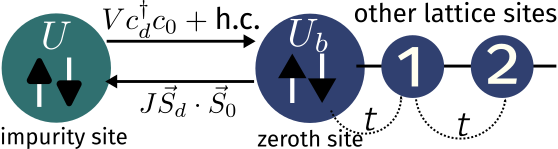
\includegraphics[width=\textwidth]{zeromode_bare.pdf}
\end{minipage}

\vspace*{\fill}
URG equations show that an \alert{attractive} \(U_b\) frustrates the zeroth site.
\[\Delta J \sim J^2 + 4U_b J \implies \text{\alert{phase transition} at }J = -4U_b\]

\vspace*{\fill}
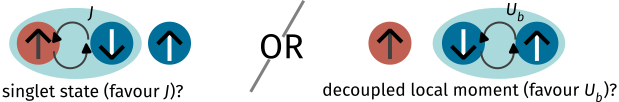
\includegraphics[width=0.9\textwidth]{frustration.pdf}\\

\vspace*{\fill}
Such a model sheds light on the Mott MIT in \(\infty-\)dimensions (as seen from DMFT).
\end{frame}

\begin{frame}{Nature of the transition}
\begin{minipage}{0.45\textwidth}
Across the transition,\\
\begin{itemize}
	\item impurity correlations vanish
	\item bath correlations become non-zero\\[10pt]
\end{itemize}

Shows that \alert{pairing correlations} in the bath are responsible for the transition.
\end{minipage}
\hspace*{\fill}
\begin{minipage}{0.5\textwidth}
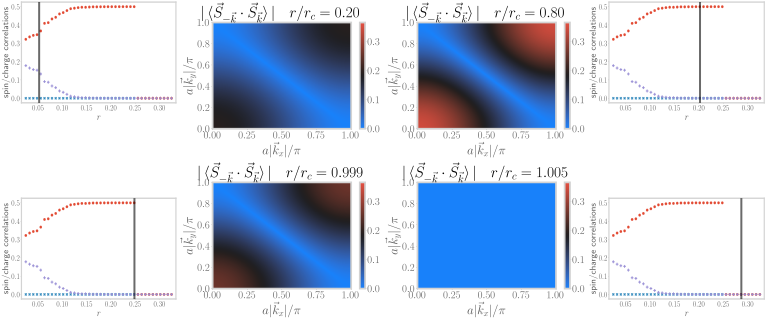
\includegraphics[width=\textwidth]{spin-charge-corr-full.pdf}
\end{minipage}

\vspace*{\fill}
The state \alert{precisely at the transition} is special:
\begin{itemize}
	\item non-Fermi liquid excitations
	\item \alert{fractional} impurity magnetisation and occupancy
\end{itemize}
\end{frame}

\section{\LARGE Holography of entanglement in 2D free fermions}
\subsection{\large Abhirup Mukherjee, Siddhartha Patra, Siddhartha Lal\\ J. Phys. A: Math. Theor. 57 275401 (2023)}

\begin{frame}{Some broad questions}
\footcite{Arias_2015,zaanen_2015}
\begin{minipage}{0.65\textwidth}
We consider 2D electrons placed on a torus in a flux \(\Phi\).
\begin{itemize}
	\item Is the entanglement content of this system \alert{holographic}?\\[10pt]
	\item Is there any \alert{topological} notion within the entanglement measures?
\end{itemize}
\end{minipage}
\hspace*{\fill}
\begin{minipage}{0.3\textwidth}
	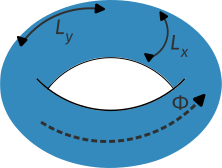
\includegraphics[width=\textwidth]{torus.pdf}
\end{minipage}

\vspace*{\fill}
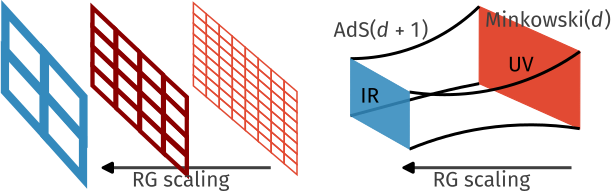
\includegraphics[width=0.8\textwidth]{holography.pdf}
\end{frame}

\begin{frame}{Results}

\begin{itemize}
	\item Choose subsystem in real space (red region)
	\item Apply \alert{coarse-graining transformations} in \(k-\)space
\end{itemize}

\vspace*{\fill}
Evolution of subspace entanglement shows interesting properties.

\vspace*{\fill}
\includegraphics[width=0.3\textwidth]{subsystem-torus.pdf}
\hspace*{\fill}
\includegraphics[width=0.5\textwidth]{coarse-graining.pdf}
\end{frame}

\begin{frame}{Results}
\footcite{van2010building}
\begin{minipage}{0.53\textwidth}
	Use mutual information \(I_2\) to define \alert{distance}.
\begin{itemize}
	\item Larger \(I_2\) \(\Longrightarrow\) smaller distance\\[10pt]
	\item Allows notion of \alert{curvature} as well.\\[10pt]
\end{itemize}
Coarse-graining transformations lead to \alert{emergent} spatial dimension
\end{minipage}
\hspace*{\fill}
\begin{minipage}{0.43\textwidth}
	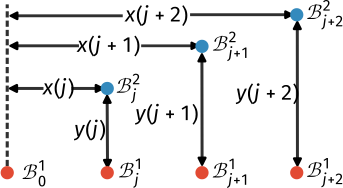
\includegraphics[width=\textwidth]{curvature-scheme.pdf}
\end{minipage}

\onslide<2>{
\vspace*{\fill}
\begin{minipage}{0.4\textwidth}
	\includegraphics[height=0.25\textheight]{Matroshka.png}
	\includegraphics[height=0.25\textheight]{nested.png}
\end{minipage}
\hspace*{\fill}
\begin{minipage}{0.55\textwidth}
Other consequences:
\begin{itemize}
	\item \alert{hierarchy} of entanglement exists along the RG
	\item hierarchy also present in \alert{multipartite entanglement}
\end{itemize}
\end{minipage}
}
\end{frame}

\begin{frame}{Results}
\footcite{oshikawa2000topological,seki2017topological,alexandradinata_2011}
\begin{minipage}{0.63\textwidth}
\begin{itemize}
	\item By tuning flux, we relate Luttinger's volume to functions of entanglement
	\item Entanglement spectral flow is also related to Chern numbers in presence of magnetic field
\end{itemize}
\end{minipage}
\hspace*{\fill}
\begin{minipage}{0.35\textwidth}
\includegraphics[width=\textwidth]{cylinder.pdf}
\end{minipage}

\vspace*{\fill}
\includegraphics[width=\textwidth]{spectral-flow.pdf}
\end{frame}

\section{\LARGE Revealing the magnetic dimensional crossover in the Heisenberg ferromagnet $\text{CrSiTe}_3$ through picosecond strain pulses}
\subsection{\large A Kumar N M, S Mukherjee,{\bf Abhirup Mukherjee}, A Punjal, S Purwar, T Setti, S Prabhu S., S Lal, N Kamaraju\\ Phys. Rev. B 111, L140414 (2025)}

\begin{frame}{GL Theory for Spin-Phonon Interaction}
	\footcite{Ron2019,Anjan2025}
	Prof. Kamaraju’s group investigated the \focus{magnetic dimensional crossover} (paramagnet $\to$ 2D short-range order $\to$ 3D long-range order) in CrSiTe$_3$ using \focus{pump-probe} spectroscopy.
	\vfill
	\begin{minipage}{0.5\textwidth}
	\centering
	\includegraphics[width=0.8\textwidth]{pumpProbe.png}
	\vfill
	\includegraphics[width=\textwidth]{MDC.png}
	\end{minipage}
	\hfill
	\begin{minipage}{0.49\textwidth}
	\begin{itemize}
		\item The acoustic strain pulses show a red-shift (\focus{softening}) of the high-frequency phonons and a \focus{gapping} out of the low-frequency phonon modes.
		\item We came up with a \focus{Ginzburg-Landau model} of phonons interacting with lattice spin fluctuations to explain these features.
			\[ \mathcal{L} = \sum_j [{\dot{Q}_j}^2 - (\lambda - M^2\chi)(Q_{j+1} - Q_j)^2 - M^2\xi Q_j^2] \]\vspace*{-15pt}
		\item Renormalisation of \focus{phonon dispersion and spring constant} due to interactions explains the softening and gapping.
	\end{itemize}
		
\end{minipage}
\end{frame}
\begin{frame}{Unitary RG Phase Diagram and Pseudogapping Transition}
\begin{minipage}{0.5\textwidth}
	\focus{Competition} between Kondo coupling and local interaction on bath sites:
\[\Delta J^{(j)}_{{\bf k}_1, {\bf k}_2} = -2\sum_{{\bf q}} \frac{J^{(j)}_{{\bf k}_2,{\bf q}} J^{(j)}_{{\bf q},{\bf k}_1} + 4J^{(j)}_{{\bf q}, {\bf \bar q}} W_{{\bf \bar q}, {\bf k}_2, {\bf k}_1, {\bf q}}}{\omega - \frac{1}{2}|\varepsilon_j| + J^{(j)}_{{\bf q}}/4 + W_{{\bf q}}/2}\]
\end{minipage}
	\hfill
\begin{minipage}{0.25\textwidth}
	\centering
	\includegraphics[width=\textwidth]{Jub.pdf}
\end{minipage}
	
\begin{center}
	\begin{minipage}{0.35\textwidth}
	\includegraphics[width=\linewidth]{phaseDiagram.pdf}
	\end{minipage}
	\hfill
	\begin{minipage}{0.6\textwidth}
	\begin{itemize}
		\item Competition leads to \focus{Kondo breakdown} for $W<0$
		\item Phase diagram shows \focus{pseudogap} phase lying between Fermi liquid (FL) and Mott insulator (MI).
		\item PG possesses non-Fermi liquid excitations -- a \focus{Mott Metal}
	\end{itemize}
	\end{minipage}
\end{center}
\end{frame}

\begin{frame}{Journey Into The Pseudogap}
	\begin{itemize}
		\item Strength of Landau quasiparticle excitations of FL (\focus{QP residue} Z) vanishes upon entering PG.
		\item Impurity magnetisation \(\langle S_d^z \rangle\) grows dramatically in PG: \focus{breakdown} of Kondo screening.
		\item Impurity-bath spin correlations vanish around antinode: signature of \focus{pseudogap}
	\end{itemize}
	\vfill
	
	\includegraphics[width=0.32\textwidth]{QPR_77-1500.pdf}
	\includegraphics[width=0.32\textwidth]{sdz_77-1500.pdf}
	\includegraphics[width=0.32\textwidth]{SF-3.pdf}
\end{frame}

\begin{frame}{Luttinger Surfaces in the Pseudogap}
	\footcite{keimer2015quantum}
	\begin{minipage}{0.75\textwidth}
	\begin{itemize}
		\item PG shows \focus{electronic differentiation} in lattice spectral function: gapped antinodal regions (\focus{Luttinger surfaces}), gapless excitations in nodal regions.
		\item Electron \focus{scattering rate}  shows divergences in gapped antinodal regions, while it is analytic in gapless nodal regions.
		\item Impurity spectral function shows \focus{pseudogap} of Fermi arcs!
	\end{itemize}
	\end{minipage}
	\hfill
	\begin{minipage}{0.2\textwidth}
	\includegraphics[width=\textwidth]{fermiArc1.png}
	\end{minipage}
	\vfill
	
	\centering
	\includegraphics[height=0.25\textwidth]{kspaceDOS-77.pdf}
	\hfill
	\includegraphics[height=0.25\textwidth]{selfEnergyKspace.pdf}
	\hfill
	\includegraphics[height=0.25\textwidth]{Ad_zoomin_77-1500.pdf}
\end{frame}

\begin{frame}{Universal Scaling of Spectral Features}
	\begin{itemize}
		\item Electron Scattering Rate of NFLs cross \focus{Mott-Ioffe-Regel (MIR) bound} (no electron-like excitations!), while FLs are within it.\\[10pt]
		\item \( 1/\Sigma^{\prime\prime} \sim 1/\Sigma^{\prime\prime}_0 + \omega^2\). Appearance of power-law exponents such as 2 signals \focus{universality}.\\[10pt]
		\item Optical Conductivity \(\sigma \sim A(\omega) \tau(\omega)\) shows a \focus{shifted ``Drude" peak}
	\end{itemize}
	\vfill
	
	\centering
	\hfill
	\includegraphics[height=0.22\textwidth]{selfEnergy_d_zoomin_77-1000withMIR.pdf}
	\hfill
	\includegraphics[height=0.22\textwidth]{selfEnergy_d_fit_77-1500.pdf}
	\hfill
	\includegraphics[height=0.22\textwidth]{sigma_in.pdf}
	\hfill
\end{frame}

\begin{frame}{Tiling Details: Greens Function}

\begin{equation}\begin{aligned}
	G( k,\sigma;\omega) =  \sum_{\nu, n} C_{\nu, k} &\left[\frac{\braket{\psi_\text{gs}({ r_d}) | \mathcal{T}_{\nu,\sigma} | \psi_{n}({ r_d})}\braket{\psi_n({ r_d}) | \mathcal{T}_{\nu,\sigma}^\dagger | \psi_\text{gs}({ r_d})}}{\omega - (E_n - E_0 + \epsilon_\nu)}\right.\\
					   &+ \left.\frac{\braket{\psi_\text{gs}({ r_d}) | \mathcal{T}^\dagger_{\nu,\sigma} | \psi_{n}({ r_d})}\braket{\psi_n({ r_d}) | \mathcal{T}_{\nu,\sigma} | \psi_\text{gs}({ r_d})}}{\omega + (E_n - E_0 - \epsilon_\nu)}\right]~.
\end{aligned}\end{equation}

\begin{equation}\begin{aligned}
	G_\text{loc}(\omega) = \mathcal{G}(d\sigma; \omega - \epsilon_\text{loc}) + \sum_{\nu} C_{\nu} \left[\mathcal{G}(\mathcal{T}_{\nu,\sigma},d\sigma; \omega - \epsilon_{\nu}) + \sum_{\bf k}\mathcal{G}(\mathcal{T}_{\nu,\sigma},\mathcal{T}_{ k,\sigma}; \omega - \epsilon_{\nu})\right] \\
	+ \sum_{ k} \mathcal{G}(d\sigma,\mathcal{T}_{ k,\sigma}; \omega) ~,
\end{aligned}\end{equation}
\end{frame}

\begin{frame}{Tiling Details: Static Correlation}
\begin{equation}\begin{aligned}
&\sum_{ r_d}\braket{\Psi_\text{gs} | c_{{ r_d +  r},\sigma}(t) c^\dagger_{{ r_d},\sigma} | \Psi_\text{gs}} \\
&= \sum_{n}F_n^*( r)\braket{\psi_\text{gs}({ r_d}) |  c_{{ r_d},\sigma}(t) | \psi_{n}( r_d)} \braket{\psi_{n}( r_d) | c^\dagger_{{ r_d},\sigma} | \psi_\text{gs}({ r_d})}\\
																													  &+ \sum_{ k, n}F^\prime_n( k)F_n^*( r)\braket{\psi_\text{gs}({ r_d}) | \mathcal{T}_{ k,\sigma}(t) | \psi_{n}( r_d)} \braket{\psi_{n}( r_d) | c^\dagger_{{ r_d},\sigma} | \psi_\text{gs}({ r_d})}\\
																													  &+ \sum_{ k, n}{F^\prime_n( k)}^*F_n^*( r)\braket{\psi_\text{gs}({ r_d}) | c_{ r_d,\sigma}(t) | \psi_{n}( r_d)} \braket{\psi_{n}( r_d) | \mathcal{T}^\dagger_{ k,\sigma} | \psi_\text{gs}({ r_d})}\\
																													  &+\sum_{ k_1, k_2}F^\prime_n( k_1){F^\prime_n( k_2)}^*F_n^*( r)\braket{\psi_\text{gs}({ r_d}) | \mathcal{T}_{ k_1,\sigma}(t) | \psi_{n}( r_d)} \braket{\psi_{n}( r_d) | \mathcal{T}^\dagger_{ k_2,\sigma} | \psi_\text{gs}({ r_d})}~,
\end{aligned}\end{equation}
\end{frame}
\end{document}

